\documentclass{beamer}
\usepackage{etex}
\usepackage{graphicx}
\usepackage[export]{adjustbox}
\usepackage{todonotes}
\usepackage{subcaption}
\usepackage{alltt}
\renewcommand{\ttdefault}{txtt}
\usepackage{ stmaryrd  }
\usepackage{ amssymb }
\usepackage{lmodern}
\usepackage{amsmath}
\newcommand*\rot{\rotatebox{45}}
\usepackage{tikz}
\usetikzlibrary{shapes,arrows,calc,positioning}
\newcommand{\tikzmark}[1]{\tikz[overlay,remember picture] \node (#1) {};}
\usepackage{multicol}
\usepackage{listings}
\usepackage{array}
\usepackage{fancyvrb}
\definecolor{lightgray}{rgb}{.9,.9,.9}
\definecolor{darkgray}{rgb}{.4,.4,.4}
\definecolor{purple}{rgb}{0.65, 0.12, 0.82}
\lstset{
  frame=none,
  xleftmargin=2pt,
  stepnumber=1,
  numbers=left,
  numbersep=5pt,
  numberstyle=\ttfamily\tiny\color[gray]{0.3},
  belowcaptionskip=\bigskipamount,
  captionpos=b,
  escapeinside={*'}{'*},
  language=haskell,
  tabsize=2,
  emphstyle={\bf},
  commentstyle=\it,
  stringstyle=\mdseries\rmfamily,
  showspaces=false,
  keywordstyle=\bfseries\rmfamily,
  columns=flexible,
  basicstyle=\tiny\sffamily,
  showstringspaces=false,
  morecomment=[l]\%,
}
%
% Choose how your presentation looks.
%
% For more themes, color themes and font themes, see:
% http://deic.uab.es/~iblanes/beamer_gallery/index_by_theme.html
%
\mode<presentation>
{
  \usetheme{default}      % or try Darmstadt, Madrid, Warsaw, ...
  \usecolortheme{whale} % or try albatross, beaver, crane, ...
  \usefonttheme{default}  % or try serif, structurebold, ...
  \setbeamertemplate{navigation symbols}{}
  \setbeamertemplate{caption}[numbered]
  \setbeamertemplate{footline}[page number]
  \setbeamercolor{block body}{bg=blue!10,fg=black}
   \setbeamercolor{block title}{bg=structure.fg, fg=white}
  %\addtobeamertemplate{block begin}{\setlength\abovedisplayskip{0pt}}
}

\usepackage[english]{babel}
\usepackage[utf8x]{inputenc}
\captionsetup{compatibility=false}

\title[SYMBOLIC TOPHAT]{A symbolic execution semantics for TopHat}
\author{Nico Naus}
\institute{\includegraphics[height=3cm,valign=t]{uulogo.png}}
\date{September 25th, 2019}

\begin{document}

\begin{frame}
  \titlepage
\end{frame}

% Uncomment these lines for an automatically generated outline.
%\begin{frame}{Outline}
%  \tableofcontents
%\end{frame}

%===================================================
%   INTRODUCTION
%===================================================
\section{Introduction}



%NOTE: Imagine you're on a navy ship. This one for example. You're standing on the bridge and the smoke detectors sound an alarm in two sections, granades are bombarding the ship, pirates are approaching, what do you do?
\section{Introduction}
\begin{frame}{}
\includegraphics[height=8cm,center]{ship.jpg}
\end{frame}

\begin{frame}{}
\begin{figure}
\begin{subfigure}[t]{0.5\textwidth}
\includegraphics[height=6cm]{rinus.jpg}\\
Prof. Rinus Plasmeijer\\
Radboud University
\end{subfigure}%
\end{figure}
%NOTE: this was one of the questions that Rinus Plasmeijer was having.
%state the goal of the presentation and the chapters
\end{frame}


%===================================================
%   ITASKS
%===================================================


\begin{frame}[fragile]{iTasks}

%first publication on iTasks from 2007, a lot of work that proceeded it, for example on generic UI
%show code for task definition here
%show examples of combinators
\pause
\begin{Verbatim}[fontsize=\small]
:: Task a :== Event → State → (Reduct a, Reponses, State)
\end{Verbatim}
\pause
%these are mondads by the way
\begin{Verbatim}[fontsize=\small]
(>>=) :: Task a → (a → Task b) → Task b
(>>*) :: Task a → [TaskStep a b] → Task b
(-||-) :: Task a → Task a → Task a
(@:) :: User → Task a → Task a
\end{Verbatim}
%and several more
\end{frame}

\begin{frame}[fragile]{iTasks}
%examples: workflow, rapid prototyping IOT
%concrete examples
\begin{Verbatim}[fontsize=\scriptsize]
shipTask :: Task SimulationState
shipTask = viewSharedInformation "ShipSimulator" [ ] shipStore
       >>* [OnAction (Action "Move"       [])
                     (always
                     (\st -> moveTask st))
           ,OnAction (Action "Pick up"    [])
                     (ifValue (hasInventory)
                     (\st -> set (applyPickup st) shipStore >>| shipTask))
           ,OnAction (Action "Extinguish" [])
                     (ifValue (canExtinguish)
                     (\st -> set (applyExtinguish st) shipStore >>| shipTask))
           ]
\end{Verbatim}
\end{frame}

\begin{frame}{iTasks}
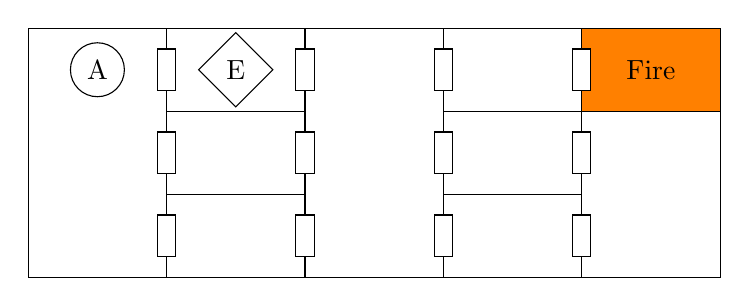
\begin{tikzpicture}[scale=2, node distance = 3em, auto]

%nodes
\node [draw, text centered, minimum height=9em,minimum width=5em,xshift=4em](1){};

\node [draw, minimum width=5em, text centered, minimum height=3em,right of=1,xshift=2em](3){};
\node [draw, minimum width=5em, text centered, minimum height=3em,above of=3](2){};
\node [draw, minimum width=5em, text centered, minimum height=3em,below of=3](4){};

\node [draw, text centered, minimum height=9em,minimum width=5em,right of = 3,xshift=2em](5){};

\node [draw, minimum width=5em, text centered, minimum height=3em,right of=5,xshift=2em](6){};
\node [draw, minimum width=5em, text centered, minimum height=3em,above of=6](7){};
\node [draw, minimum width=5em, text centered, minimum height=3em,below of=6](8){};

\node [draw, minimum width=5em, text centered, minimum height=3em,right of=7,xshift=2em, fill=orange](9){};
\node [draw, minimum width=5em, text centered, minimum height=6em,below of=9,yshift=-1.5em](10){};

\node[circle, draw, text centered, minimum height = 1em, left of=2, xshift=-2em](alice){A};
\node[diamond, draw, text centered, minimum height = 1em, right of=2, xshift=-3em](extinguisher){E};
\node[, text centered, minimum height = 1em, right of=7, xshift=2em](fire){Fire};


%doors

\node [draw, text centered, minimum height=1.5em,minimum width=0.05em,left of=2, xshift=0.5em, fill=white](11){};
\node [draw, text centered, minimum height=1.5em,minimum width=0.05em,left of=3, xshift=0.5em, fill=white](11){};
\node [draw, text centered, minimum height=1.5em,minimum width=0.05em,left of=4, xshift=0.5em, fill=white](11){};

\node [draw, text centered, minimum height=1.5em,minimum width=0.05em,right of=2, xshift=-0.5em, fill=white](11){};
\node [draw, text centered, minimum height=1.5em,minimum width=0.05em,right of=3, xshift=-0.5em, fill=white](11){};
\node [draw, text centered, minimum height=1.5em,minimum width=0.05em,right of=4, xshift=-0.5em, fill=white](11){};



\node [draw, text centered, minimum height=1.5em,minimum width=0.05em,left of=6, xshift=0.5em, fill=white](11){};
\node [draw, text centered, minimum height=1.5em,minimum width=0.05em,left of=7, xshift=0.5em, fill=white](11){};
\node [draw, text centered, minimum height=1.5em,minimum width=0.05em,left of=8, xshift=0.5em, fill=white](11){};

\node [draw, text centered, minimum height=1.5em,minimum width=0.05em,left of=9, xshift=0.5em, fill=white](11){};
\node [draw, text centered, minimum height=1.5em,minimum width=0.05em,right of=6, xshift=-0.5em, fill=white](11){};
\node [draw, text centered, minimum height=1.5em,minimum width=0.05em,right of=8, xshift=-0.5em, fill=white](11){};

\end{tikzpicture}

\begin{itemize}
\item Move
\item Pick up
\item Extinguish
\end{itemize}


\end{frame}

\begin{frame}{Research Questions}
%how to define & guarantee properties of tasks
%hwat kind of runtime feedback do we need to provide to end users and managers
%what is the best way of working

%or in other words: can we say more about tasks?
\begin{figure}
\begin{subfigure}[t]{0.5\textwidth}
\includegraphics[height=6cm]{rinus.jpg}\\
Prof. Rinus Plasmeijer\\
Radboud University
\end{subfigure}\pause%
\begin{subfigure}[t]{0.5\textwidth}
\includegraphics[height=6cm]{johan.jpg}\\
Prof. Johan Jeuring\\
Utrecht University
\end{subfigure}
\end{figure}

%johan has a background in ITS, and the problem looked similar.
\end{frame}


%===================================================
%   The Vision
%===================================================






\begin{frame}{The Vision}

%we look at these questions, they sound very similar: Feedback, best way of working, testing, simulation.
%iTasks can be seen as a rule based system just like a tutor: Rules, effects, state, combinartors
%inspiration
%todo: explain this with a picture
%best way of working
\pause
\begin{tikzpicture}[scale=2, node distance = 5em, auto]

%nodes
\node [draw, text centered](1){State};

\node [draw, text centered, right of=1,xshift=2cm](2){Structure};
\node [draw, text centered, below of=2](3){Rules};
\node [draw, text centered, below of=3](4){Effect};

\node [draw, text centered, right of = 2,xshift=2cm](5){Goal};

%arrows


\path [draw] (2) -- (3);
\path [draw] (3) -- (4);

\end{tikzpicture}

\end{frame}

\begin{frame}{The Vision - In practice}
%tell something about wich components we will need
% Generic feedback framework, simulator, testing framework, feedback viewer

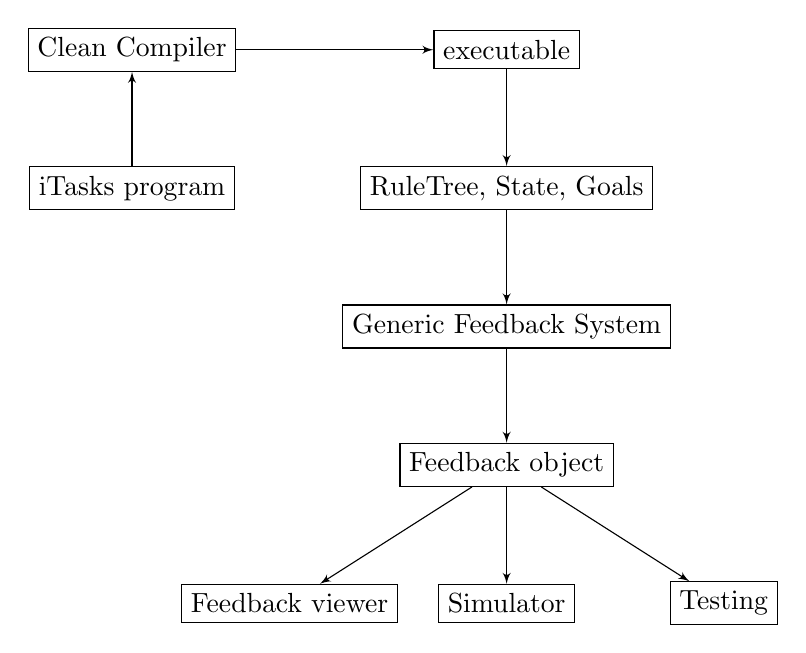
\begin{tikzpicture}[scale=2, node distance = 5em, auto]

%nodes
\node [draw, text centered](1){iTasks program};

\node [draw, text centered, above of=1](2){Clean Compiler};
\node [draw, text centered, right of=2,xshift=3cm](3){executable};
\onslide<2->{\node [draw, text centered, below of=3](4){RuleTree, State, Goals};}

\onslide<3->{\node [draw, text centered, below of = 4](5){Generic Feedback System};}

\onslide<4->{\node [draw, text centered, below of=5](6){Feedback object};}

\onslide<6->{\node [draw, text centered, below of=6](8){Simulator};}
\onslide<5->{\node [draw, text centered, left of=8,xshift=-1cm](7){Feedback viewer};}

\onslide<6->{\node [draw, text centered, right of=8,xshift=1cm](9){Testing};}

%arrows

\path [draw, -latex'] (1) -- (2);
\path [draw, -latex'] (2) -- (3);
\onslide<2->{\path [draw, -latex'] (3) -- (4);}
\onslide<3->{\path [draw, -latex'] (4) -- (5);}
\onslide<4->{\path [draw, -latex'] (5) -- (6);}
\onslide<5->{\path [draw, -latex'] (6) -- (7);}
\onslide<6->{\path [draw, -latex'] (6) -- (8);}
\onslide<6->{\path [draw, -latex'] (6) -- (9);}

\end{tikzpicture}
\end{frame}

%===================================================
%   The story so far
%===================================================

\begin{frame}{So far}
%first sub problem: Generic feedback framework: Any rule based system, DSL to capture rule & effect, algorithms, multi user, labels
%put some TFP slides here, name publication
%mention current extension

\end{frame}

\begin{frame}{Generic end-user feedback system}
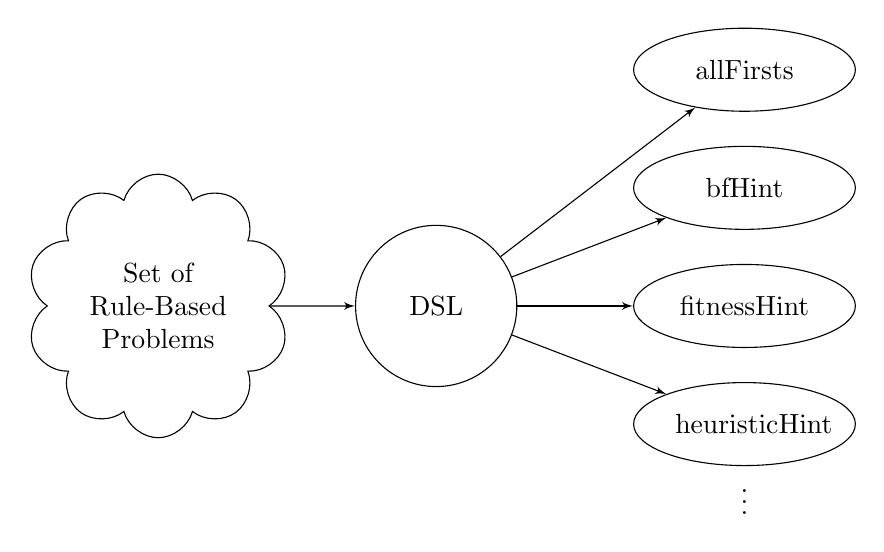
\begin{tikzpicture}[scale=1, node distance = 1.5cm, auto]

%nodes
\node [cloud, draw, text width=5em, text centered, minimum height=3em](problems){Set of Rule-Based Problems};\pause
\node [circle, draw,text width=5em, text centered, minimum height=4em,right of=problems](dsl)[right=1cm]{DSL};
%lines

\path [draw, -latex'] (problems) -- (dsl);\pause

\node [ellipse, draw,text width=5em, text centered, minimum height=3em,right of=dsl](fitness)[right=1cm]{fitnessHint};
\node [ellipse, draw,text width=5em, text centered, minimum height=3em,above of=fitness](bf){bfHint};
\node [ellipse, draw,text width=5em, text centered, minimum height=3em,above of=bf](allFirsts){allFirsts};
\node [ellipse, draw,text width=5em, text centered, minimum height=3em,below of=fitness](heuristic){heuristicHint};
\node [draw=none, text width=5em, text centered, minimum height=2em,below of=heuristic](dots2)[below=-1cm]{\vdots};

\path [draw, -latex'] (dsl) -- (fitness);
\path [draw, -latex'] (dsl) -- (bf);
\path [draw, -latex'] (dsl) -- (allFirsts);
\path [draw, -latex'] (dsl) -- (heuristic);

\end{tikzpicture}
\end{frame}

\begin{frame}{DSL}

\begin{figure}
\begin{subfigure}[t]{0.5\textwidth}
\begin{align*}
\onslide<2->{State      &::  a}\\
\onslide<3->{Rule       &::  Rule\ Name\ Effect}\\
\onslide<3->{Name       &::  String\\
Effect     &::  a \rightarrow a}\\
\onslide<5->{Goal       &::  Predicate\\
Predicate  &::  a \rightarrow Bool}
\end{align*}
\end{subfigure}%
\begin{subfigure}[t]{0.5\textwidth}
\begin{align*}
\onslide<4->{:: RuleTree  &= Seq\ [RuleTree]\\
          &\ |\ Choice\ [RuleTree]\\
          &\ |\ Parallel\ [RuleTree]\\
          &\ |\ Condition\ Predicate\\ & \hspace{2cm}RuleTree\\
          &\ |\ Leaf\ Rule\\
          &\ |\ Empty}
\end{align*}
\end{subfigure}
\end{figure}
\end{frame}

\begin{frame}[fragile]{DSL - Example}
\begin{Verbatim}[fontsize=\scriptsize]
shipSimulation :: RuleTree SimulationState
shipSimulation =
  Seq
    [ Choice [ Choice (map (\x -> Condition (isValidMove x)
                                            (Rule (Rule (toString x)
                                                        (applyMove x))))
                           [1..10])
             , Condition hasInventory (Rule (Rule "Pickup" applyPickup))
             , Condition canExtinguish (Rule (Rule "extinguish"
                                                   applyExtinguish))
             ]
    , shipSimulation
    ]
\end{Verbatim}
\pause
\begin{Verbatim}[fontsize=\scriptsize]
shipNotOnFire :: SimulationState -> Bool
shipNotOnFire {ship} = not (foldr (||) False (map (onFire) (flatten ship)))
\end{Verbatim}
\end{frame}


\begin{frame}[fragile]{Solving algorithms}

\begin{Verbatim}[fontsize=\large]
allFirsts :: (RuleTree a) a -> [Name]
\end{Verbatim}
\begin{Verbatim}[fontsize=\large]
fitnessHint :: (a -> Int) (RuleTree a) a -> [Name]
\end{Verbatim}
\begin{Verbatim}[fontsize=\large]
bfHint :: (a -> Bool) (RuleTree a) a -> [Name]
\end{Verbatim}

\end{frame}



\begin{frame}[fragile]{Feedback generation - Example}
\begin{Verbatim}[fontsize=\normalsize]
shipSimulation :: RuleTree SimulationState

shipNotOnFire :: SimulationState -> Bool

\end{Verbatim}
\pause
\begin{Verbatim}[fontsize=\normalsize]
hint :: SimulationState -> [Name]
hint = bfHint shipNotOnFire shipSimulation
\end{Verbatim}
\end{frame}


\begin{frame}{DSL}
\begin{figure}
\begin{align*}
:: RuleTree  &= Seq\ [RuleTree]\\
          &\ |\ Choice\ [RuleTree]\\
          &\ |\ Parallel\ [RuleTree]\\
          &\ |\ Condition\ Predicate\ RuleTree\\
          &\ |\ Leaf\ Rule\\
          &\ |\ Empty\\
          \onslide<2->{&\ |\ Assign\ User\ RuleTree\\
          &\ |\ Label\ String\ RuleTree}
\end{align*}
\end{figure}
\end{frame}

%===================================================
%   Future work
%===================================================

\begin{frame}{Future work}
%applying to full itasks
%this requires bookkeeping  (algorithms and goals), and RuleTree generation (maybe show tonic pictures?)
%support for sumulation, testing, verification
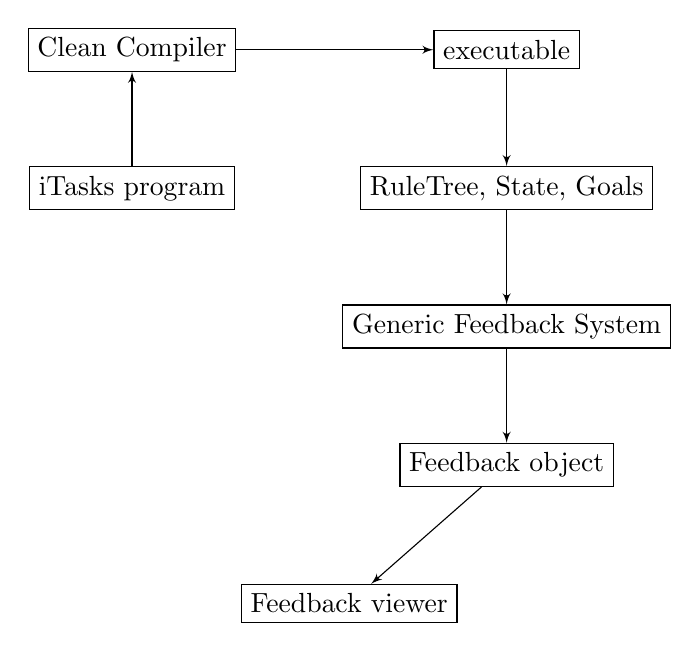
\begin{tikzpicture}[scale=2, node distance = 5em, auto]

%nodes
\node [draw, text centered](1){iTasks program};

\node [draw, text centered, above of=1](2){Clean Compiler};
\node [draw, text centered, right of=2,xshift=3cm](3){executable};
\onslide<2->{\node [draw, text centered, below of=3](4){RuleTree, State, Goals};}

\node [draw, text centered, below of = 4](5){Generic Feedback System};

\node [draw, text centered, below of=5](6){Feedback object};

\onslide<2->{\node [draw, text centered, below of=6,xshift=-2cm](7){Feedback viewer};}

%arrows

\path [draw, -latex'] (1) -- (2);
\path [draw, -latex'] (2) -- (3);
\onslide<2->{\path [draw, -latex'] (3) -- (4);
\path [draw, -latex'] (4) -- (5);}
\path [draw, -latex'] (5) -- (6);
\onslide<2->{\path [draw, -latex'] (6) -- (7);}


\end{tikzpicture}
\end{frame}


\begin{frame}{Future work - iTasks integration}
\Large
\begin{align*}
\text{Task} &\rightarrow \text{Rule}\\
\onslide<2->{\text{T}_1 >\!\!>\!= (\text{T}_2 -\!\!||\!\!- \text{T}_3)} \onslide<3->{&\rightarrow \text{Seq } [\text{R}_1,  \text{Parallel } [\text{R}_2,\text{R}_3]]\\}
\onslide<4->{\text{T}_1^* >\!\!>\!= (\text{T}_2 -\!\!||\!\!- \text{T}_3^*)} \onslide<5->{&\rightarrow \text{Seq } [\text{R}_1,\text{R}_3]}
\end{align*}

\end{frame}


\begin{frame}{Future work}
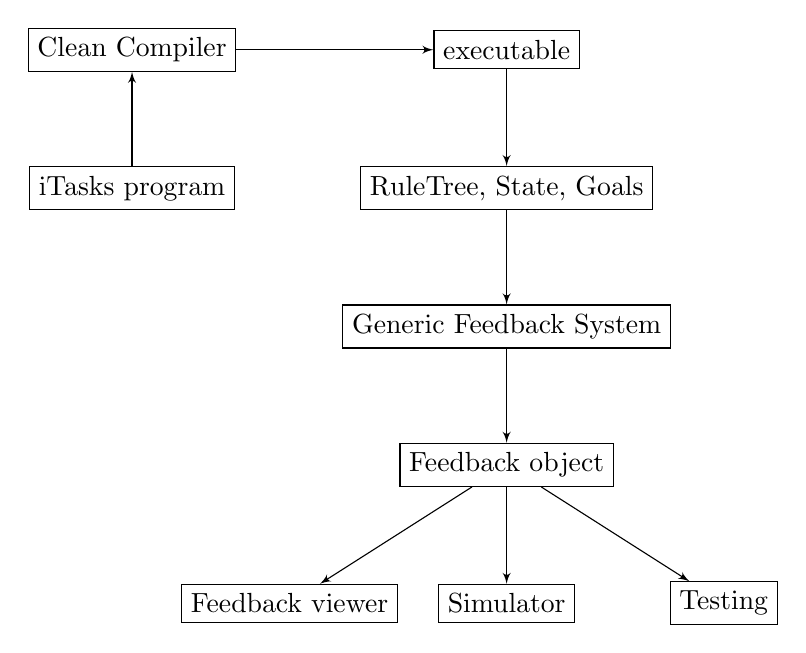
\begin{tikzpicture}[scale=2, node distance = 5em, auto]

%nodes
\node [draw, text centered](1){iTasks program};

\node [draw, text centered, above of=1](2){Clean Compiler};
\node [draw, text centered, right of=2,xshift=3cm](3){executable};
\node [draw, text centered, below of=3](4){RuleTree, State, Goals};

\node [draw, text centered, below of = 4](5){Generic Feedback System};

\node [draw, text centered, below of=5](6){Feedback object};

\onslide<2->{\node [draw, text centered, below of=6](8){Simulator};}
\node [draw, text centered, left of=8,xshift=-1cm](7){Feedback viewer};

\onslide<2->{\node [draw, text centered, right of=8,xshift=1cm](9){Testing};}

%arrows

\path [draw, -latex'] (1) -- (2);
\path [draw, -latex'] (2) -- (3);
\path [draw, -latex'] (3) -- (4);
\path [draw, -latex'] (4) -- (5);
\path [draw, -latex'] (5) -- (6);
\path [draw, -latex'] (6) -- (7);
\onslide<2->{\path [draw, -latex'] (6) -- (8);}
\onslide<2->{\path [draw, -latex'] (6) -- (9);}

\end{tikzpicture}
\end{frame}


\begin{frame}{Future work - Simulation \& Testing}
\Large
\begin{align*}
\text{Task} &\rightarrow \text{Rule}\\
\text{T}_1 >\!\!>\!= (\text{T}_2 -\!\!||\!\!- \text{T}_3) &\rightarrow \text{Seq } [\text{R}_1,  \text{Parallel } [\text{R}_2,\text{R}_3]]\\
\text{T}_1^* >\!\!>\!= (\text{T}_2 -\!\!||\!\!- \text{T}_3^*) &\rightarrow \text{Seq } [\text{R}_1,\text{R}_3]\\
\onslide<2->{\text{T}_1^* >\!\!>\!= (\text{T}_2 -\!\!||\!\!- \text{T}_3^*)} \onslide<3->{&\rightarrow \text{Seq } [\text{R}_1,  \text{Parallel } [\text{G}_2,\text{R}_3]]}
\end{align*}


\end{frame}
%===================================================
%  CONCLUSION
%===================================================
\section{Conclusion}


\begin{frame}
\includegraphics[height=1.5cm]{itasks.png}\\
http://wiki.clean.cs.ru.nl/itasks\\
\vspace{0.5cm}
\includegraphics[height=1.5cm]{ideas.png}\\
http://ideas.cs.uu.nl/\\
\vspace{1cm}
http://niconaus.nl\\
%TODO: insert further reading references

\end{frame}

%NOTE: Remember, we were on a navy ship, what do we do? We make a generic feedback system.

%===================================================
%  APPENDIX
%===================================================
\section*{Appendix}
\appendix

\end{document}
